% Printed 92--101. Continuation from printed 91.
\clearpage
\noindent 92\hfill NACHLASS.\hfill\mbox{}\par
\[
\begin{aligned}
\varphi_1+\tfrac12t&=\varphi\\
\sqrt{(1-ee\sin\varphi^2)}&=k
\end{aligned}
\]
gesetzt wird, und $a_0$ die halbe grosse Axe bezeichnet:
\[
\begin{aligned}
a'&=\frac{a_0(1-ee)}{k^3}\\
b'&=a'\cdot\frac{3ee\sin\varphi\cos\varphi}{kk}\\
c'&=a'\cdot\frac{3ee}{k^4}(1-(2-4ee)\sin\varphi^2-3ee\sin\varphi^4)
\end{aligned}
\]
und
\[
\begin{aligned}
\alpha'&=\frac{a_0\cos\varphi}{k}\quad\bigg]\\
-\beta'&=a'\sin\varphi\\
-\gamma'&=a'\cos\varphi+b'\sin\varphi\\
-\delta'&=-a'\sin\varphi+2b'\cos\varphi+c'\sin\varphi.
\end{aligned}
\]
[Damit ergibt sich:
\[
\begin{aligned}
-r\cos A&=a't\{1+\tfrac1{24}\tfrac{c'}{a'}tt-(\tfrac1{12}\tfrac{a'}{\alpha'}\cos\varphi+\tfrac18\sin\varphi^2)\lambda\lambda\}\\
r\sin A&=\alpha'\lambda\{1+(\tfrac1{24}\tfrac{a'}{\alpha'}\cos\varphi-\tfrac18\tfrac{b'}{\alpha'}\sin\varphi)tt-\tfrac1{24}\sin\varphi^2\cdot\lambda\lambda\}\\
\Delta&=\lambda\sin\varphi\{1+(-\tfrac1{24}+\tfrac16\tfrac{a'}{\alpha'}\cos\varphi+\tfrac1{12}\tfrac{b'}{a'}\operatorname{cotang}\varphi)tt+\tfrac1{12}\tfrac{\alpha'}{a'}\cos\varphi\cdot\lambda\lambda\}
\end{aligned}
\]
oder
\[
\begin{aligned}
-r\cos A&=\frac{a_0(1-ee)}{k^3}t\bigg\{1+\frac{ee}{8k^4}(1-(2-4ee)\sin\varphi^2-3ee\sin\varphi^4)tt\\
&\hspace{20mm}-\frac{1}{24(1-ee)}(2+(1-5ee)\sin\varphi^2+2ee\sin\varphi^4)\lambda\lambda\bigg\}\\
r\sin A&=\frac{a_0\cos\varphi}{k}\lambda\{1+\frac{1}{24k^4}(1-ee)(1-10ee\sin\varphi^2)tt-\tfrac1{24}\sin\varphi^2\cdot\lambda\lambda\}\\
\Delta&=\lambda\sin\varphi\{1+\frac{1}{24kk}(3+2ee-5ee\sin\varphi^2)tt+\frac{kk}{12(1-ee)}\cos\varphi^2\cdot\lambda\lambda\}.]
\end{aligned}
\]
\begin{center}[10.]\end{center}
Vollkommen genaue Formeln für ein Dreieck auf dem elliptischen Sphäroid.
\begin{quote}
$\varphi,\varphi'$ Polhöhen; $L,L+\lambda$ Längen zweier Örter $P,P'$\\
$a$ Radius des Erdäquators; $e$ Excentricität
\end{quote}

\clearpage
\noindent\mbox{}\hfill GEODÄTISCHE LINIE.\hfill 93\par
\begin{quote}
$A,A'$ [nordöstliche] Azimuthe [der Verticalschnitte] der Örter $P'$ bezw.\ $P$ in $P$ bezw.\ $P'$\\
$h,h'$ Höhen derselben Örter über dem Niveau\\
$K$ Chorde zwischen den beiden auf das Niveau projicirten Örtern
\end{quote}
\[
\rho=(1-ee\sin\varphi^2)^{-\frac12},\quad\rho'=(1-ee\sin\varphi^{\prime2})^{-\frac12}.
\]
[Man bilde ein] sphärisches Dreieck [dessen]
\begin{center}
\begin{tabular}{cc}
Seiten&Winkel\\
$90^\circ-\varphi$&$360^\circ-B'$\\
$90^\circ-\varphi'$&$B$\\
$\Delta$&$\lambda$
\end{tabular}
\end{center}
[Dann ist]
\[
\begin{aligned}
\operatorname{cotang}B&=\operatorname{cotang}A+\frac{\cos\varphi}{\cos\varphi'\sin\lambda}\cdot\frac{ee(\rho'\sin\varphi'-\rho\sin\varphi)}{\rho'+\dfrac{h'}a}\\
\operatorname{cotang}B'&=\operatorname{cotang}A'+\frac{\cos\varphi'}{\cos\varphi\sin\lambda}\cdot\frac{ee(\rho'\sin\varphi'-\rho\sin\varphi)}{\rho+\dfrac ha}.
\end{aligned}
\]
[Ferner ist]
\[
K=a\sqrt{\{2-2\rho\rho'(\cos\varphi\cos\varphi'\cos\lambda+(1-ee)\sin\varphi\sin\varphi)-ee(1-ee)(\rho'\sin\varphi'-\rho\sin\varphi)^2\}}.
\]
\begin{center}[11.]\end{center}
\begin{center}[Übertragung der geographischen Lage vermittelst der Sehne und des Azimuths des Verticalschnittes.]\end{center}
\begin{quote}
$\varphi$ Polhöhe eines Orts $p$; $x=\cos\varphi$, $y=\sin\varphi$, $\rho=\dfrac1{\sqrt{(1-ee\sin\varphi^2)}}$\\
Dasselbe für den Beobachtungsort $P$: $\Phi,X,Y,\mathrm P$\\
$\lambda$ Längenunterschied der Örter $p$ und $P$, positiv, wenn $P$ westlich [von $p$ liegt]\\
$K$ Chorde\\
$\delta$ Depression von $P$ in $p$\\
$A$ [südwestliches] Azimuth [der Verticalebene in $p$ nach $P$].
\end{quote}
\[
\begin{aligned}
\mathrm PX\cos\lambda-\rho x&=\frac Ka y\mathop{\dot{\mathrm c}\mathrm{os}}\delta\cos A-\frac Ka x\sin\delta\\
\mathrm PX\sin\lambda&=\frac Ka\cos\delta\sin A\\
(1-ee)(\mathrm PY-\rho y)&=-\frac Ka x\cos\delta\cos A-\frac Ka y\sin\delta.
\end{aligned}
\]

\clearpage
\noindent 94\hfill NACHLASS.\hfill\mbox{}\par
\begin{center}[12.]\end{center}
\begin{center}[Der Unterschied zwischen dem geodätischen und dem beobachteten Azimuth.]\end{center}
Ist $V=0$ die Gleichung einer Fläche, deren Punkte die Coordinaten $x,y,z$ haben, wo $V$ eine gegebene Funktion von $x,y,z$ ist, ferner $\mathrm ds=\sqrt{(\mathrm dx^2+\mathrm dy^2+\mathrm dz^2)}$, so ist, $\mathrm ds$ als constant betrachtet, für die kürzeste Linie auf dieser Fläche
\[
\frac{\mathrm ddx}{\dfrac{\mathrm dV}{\mathrm dx}}=\frac{\mathrm ddy}{\dfrac{\mathrm dV}{\mathrm dy}}=\frac{\mathrm ddz}{\dfrac{\mathrm dV}{\mathrm dz}}.
\]
Ich nehme an, dass im Anfangspunkt der Coordinaten die Ebene der $x,y$ zugleich berührende Ebene der Fläche sei, und dass die kürzeste Linie von diesem Punkt ausgehe.

Man hat dann, den Halbmesser der Krümmung in der Ebene der $x,z$ gleich $R$, den\textperiodcentered\ Halbmesser der Krümmung in der Ebene der $y,z$ gleich $R'$ gesetzt und angenommen, dass dies resp.\ die äussersten Krümmungshalbmesser sind,
\[
V=z+\frac{xx}{2R}+\frac{yy}{2R'}+\ldots\ [=0],
\]
[und wenn] ferner das Azimuth der kürzesten Linie im Anfangspunkt der Coordinaten gleich $\zeta$ gesetzt wird:
\[
\begin{array}{rclcl}
x=&s\cos\zeta&*&-s^3\dfrac{\cos\zeta}{6R}\left(\dfrac{\cos\zeta^2}{R}+\dfrac{\sin\zeta^2}{R'}\right)\ldots\\[4pt]
y=&s\sin\zeta&*&-s^3\dfrac{\sin\zeta}{6R'}\left(\dfrac{\cos\zeta^2}{R}+\dfrac{\sin\zeta^2}{R'}\right)\ldots\\[4pt]
z=&*&\multicolumn{2}{l}{-ss\left(\dfrac{\cos\zeta^2}{2R}+\dfrac{\sin\zeta^2}{2R'}\right)-\ldots\ .}
\end{array}
\]
Beim Ellipsoid setzen wir
\[
\begin{aligned}
\frac1R&=\sqrt{(aa\cos\varphi^2+bb\sin\varphi^2)}\cdot\left(\frac{\cos\varphi^2}{bb}+\frac{\sin\varphi^2}{aa}\right)=\frac{(1-ee\sin\varphi^2)^{\frac32}}{a(1-ee)}\\
\frac1{R'}&=\sqrt{(aa\cos\varphi^2+bb\sin\varphi^2)}\cdot\left(\frac{\cos\varphi^2}{aa}+\frac{\sin\varphi^2}{aa}\right)=\frac{(1-ee\sin\varphi^2)^{\frac12}}a\\
\frac1\rho&=\frac1a\left(1+\frac{ee}{1-ee}\cos\varphi^2\cos\zeta^2\right)\sqrt{(1-ee\sin\varphi^2)}.
\end{aligned}
\]
[Auf dem Rotationsellipsoid ist, wenn das] beobachtete Azimuth $=\mathfrak Z$,

\clearpage
\noindent\mbox{}\hfill GEODÄTISCHE LINIE.\hfill 95\par
\[
\zeta=\mathfrak Z-\tfrac1{12}\frac{ss}{aa}\sin2\zeta\frac{ee\cos\varphi^2(1-ee\sin\varphi^2)}{1-ee}\left(1+\frac{ee\cos\varphi^2}{1-ee}\cos\zeta^2\right).
\]
Allgemein [wird], wenn
\[
z=axx+2bxy+cyy+ex^3+3fxxy+3gxyy+hy^3+\ldots
\]
[und $\theta$ der Winkel ist, den die geodätische Linie mit der $x$-Axe bildet,]
\[
\begin{array}{rcll}
x=&s\cos\theta&*&-\tfrac23s^3(a\cos\theta+b\sin\theta)(a\cos\theta^2+2b\cos\theta\sin\theta+c\sin\theta^2)\ldots\\
y=&s\sin\theta&*&-\tfrac23s^3(b\cos\theta+c\sin\theta)(a\cos\theta^2+2b\cos\theta\sin\theta+c\sin\theta^2)\ldots\\
z=&*&\multicolumn{2}{l}{ss(a\cos\theta^2+2b\cos\theta\sin\theta+c\sin\theta^2)}\\
&&&+s^3(e\cos\theta^3+3f\cos\theta^2\sin\theta+3g\cos\theta\sin\theta^2+h\sin\theta^3)\ldots\ .
\end{array}
\]
[Hieraus folgt für das Bogenelement $\sigma$ der einer beliebigen Curve auf der Fläche
\[
\mathrm d\sigma^2=\mathrm ds^2+mm\,\mathrm d\theta^2]
\]
\[
m=s+\tfrac23s^3(bb-ac)\ldots\ .
\]
\begin{center}[13.]\end{center}
\begin{center}[Reduction des astronomischen Azimuthes auf das geodätische.]\end{center}
Die Correction des beobachteten Azimuthes $\theta$ wegen der Höhe $h$ des Objects wird [angenähert]
\[
\begin{aligned}
P&=\frac h{2a\rho}\frac{ee}{1-ee}\sin2\theta\cos\varphi^2\sqrt{(1-ee\sin\varphi^2)}\\
&=\tfrac12B\frac{ee}{1-ee}h\cos\varphi^2\sin2\theta
\end{aligned}
\]
[$\log B$ ist aus der Tabelle auf S.\ 84 zu entnehmen].

Correction [des beobachteten Azimuthes auf das Azimuth] der kürzesten Linie:
\[
-\tfrac1{12}\frac{ss}{aa\rho}\sin2\theta\frac{ee\cos\varphi^2(1-ee\sin\varphi^2)}{1-ee}=-Q
\]
\[
\left[\rho=\frac1{206\,264{,}8\ldots}\right].
\]
[Also ist angenähert]
\[
Q=\tfrac16\frac{ss}{ha}P.
\]
\begin{center}\rule{.18\textwidth}{.4pt}\end{center}

\clearpage
\noindent 96\hfill BEMERKUNGEN.\hfill\mbox{}\par
\vspace{12mm}
\begin{center}\textbf{BEMERKUNGEN.}\end{center}
{\small
Die Notizen [1] und [3] fanden sich auf einzelnen Blättern; sie sind wahrscheinlich, ebenso wie auch [2], am Ende des zweiten Jahrzehnts im vergangenen Jahrhundert entstanden. [2] ist einem Handbuche entnommen; die in dem Beispiele erwähnten Punkte Kirchhesepe und Queckenberg gehören der hannoverschen Landesvermessung an. Im Beispiele selbst sind einige Rechnungsungenauigkeiten richtig gestellt worden, wodurch die Position von Queckenberg von dem durch \textsc{Gauss} erhaltenen Werthe etwas abweicht.

Die Formeln zur indirecten Bestimmung von $\varphi'-\varphi$, $R'-R$ und $\Delta P$ unter [2] erhält man leicht aus den \textsc{Gauss}schen Gleichungen:
\[
\begin{aligned}
\cos R^*\sin\tfrac12\Delta Q&=\sin\tfrac12(\varphi'-\varphi)\cos\tfrac12\Delta P\\
\cos\tfrac12(R'-R)\cos\tfrac12\Delta Q&=\cos\tfrac12(\varphi'-\varphi)\cos\tfrac12\Delta P\\
\sin R^*\sin\tfrac12\Delta Q&=\cos\varphi^*\sin\tfrac12\Delta P\\
\sin\tfrac12(R'-R)\cos\tfrac12\Delta Q&=\sin\varphi^*\sin\tfrac12\Delta P,
\end{aligned}
\]
wenn man berücksichtigt, dass für kleine Winkel angenähert
\[
\sin x=x\cos x^{\frac13},\qquad\operatorname{tang}x=x\sec x^{\frac13}
\]
ist. Aus der ersten Gleichung folgt
\[
\varphi'-\varphi=\frac{\cos R^*}{\cos\tfrac12\Delta P}\left(\frac{\cos\tfrac12\Delta Q}{\cos\tfrac12(\varphi'-\varphi)}\right)^{\frac13}\Delta Q,
\]
und daher mit Hülfe der zweiten Gleichung:
\[
\varphi'-\varphi=\cos R^*\cdot\Delta Q(\sec\tfrac12(R'-R)\sec\tfrac12\Delta P^2)^{\frac13}.
\]
$R'-R$ ergibt sich aus der 4. und 3. Gleichung:
\[
\begin{aligned}
\sin\tfrac12(R'-R)&=\operatorname{tang}\varphi^*\sin R^*\operatorname{tang}\tfrac12\Delta Q\\
R'-R&=\operatorname{tang}\varphi^*\sin R^*\cdot\Delta Q(\sec\tfrac12(R'-R)\sec\tfrac12\Delta Q^2)^{\frac13}.
\end{aligned}
\]
Die angegebenen Werthe für $\Delta P$ findet man aus der 3. Gleichung und aus der 3. und 2. Gleichung.

Die Schlussformel für $\mathrm d\lambda$ in der Notiz [3] lautet im Original
\[
\mathrm d\lambda=\mathrm dl-\tfrac12\frac{ee}{\cos I}\cdot\mathrm d\sigma\{1-\tfrac12ee(1-\cos\sigma^2\sin I^2)+etc.\}.
\]
Die Formeln unter [4] waren von \textsc{Gauss} auf die letzte Seite seines Exemplars der »Mathematischen Abhandlungen von Dr.\ H.\ F.\ \textsc{Scherk}, Berlin, 1825«, eingetragen; die dazu gehörige Tabelle, die sich von $47^\circ$--$55^\circ$ erstreckt, und von der S.\ 82 eine Probe gibt, befand sich auf losen Blättern. Für $\log(-H)$ ist noch eine auf 7 Stellen berechnete Tabelle für dasselbe Intervall vorhanden. Wahrscheinlich sind diese Formeln zur geodätischen Übertragung, die vielleicht durch ein besonderes Verfahren erhalten wurden, vor den etwas einfacheren der »Untersuchungen über Gegenstände der höhern Geodäsie«, Art.\ 23--25 oder Art.\ 30--33,
\par}

\clearpage
\noindent\mbox{}\hfill GEODÄTISCHE LINIE.\hfill 97\par
{\small
\noindent entstanden. Man erhält aus ihnen die letztern, wenn man berücksichtigt, dass für die Glieder in den Klammern
\[
\begin{aligned}
(1-ee\sin\varphi^2)\frac{ss}{aa}+\Delta\zeta^2&=\left(\frac{1-ee}{1-ee\sin\varphi^2}\right)^2\Delta\varphi^2+\Delta\lambda^2\\
\Delta\zeta^2&=\Delta\lambda^2\sin\varphi^2,
\end{aligned}
\]
also
\[
\frac{1-3ee+2ee\sin\varphi^2}{24(1-ee)}\Delta\zeta^2=\tfrac1{24}\Delta\zeta^2-\frac{ee\sin\varphi^2(1-ee\sin\varphi^2)ss}{12(1-ee)aa}+\frac{ee(1-ee)\sin\varphi^2}{12(1-ee\sin\varphi^2)^2}\Delta\varphi^2
\]
und
\[
\frac{1-ee\sin\varphi^2}{12(1-ee)}\Delta\lambda^2=\tfrac1{12}\Delta\zeta^2+\frac{1-ee\sin\varphi^2}{12(1-ee)}\frac{ss}{aa}-\frac{1-ee}{12(1-ee\sin\varphi^2)^2}\Delta\varphi^2
\]
ist. Hierbei ist zu $\Delta\varphi$, $\Delta\lambda$, $\Delta\zeta$ der Factor $\rho=\dfrac1{206\,265}$ zuzufügen.

Die Formeln [4] sind von \textsc{Gauss} zur Berechnung der geodätischen Positionen seiner Hauptdreieckspunkte benutzt worden; Breite, Länge und Azimuth wurden von Göttingen, Sternwarte, aus von Punkt zu Punkt übertragen. Das den Formeln beigefügte Beispiel ist diesen Rechnungen entnommen, die sich auf den letzten Seiten eines Beobachtungs- und Rechnungsheftes für die Gradmessung aus dem Jahre 1825 befinden. Die Bezeichnungen sind in dem Beispiel zugesetzt worden.

Die unter [5] mitgetheilten Formeln, die einem Handbuche entstammen, sind Annäherungen an die Formeln [4]. Zu ihnen gehört eine von $50^\circ$ bis $54^\circ$ sich erstreckende, auf dem Abplattungswerthe $\dfrac1{302{,}78}$ beruhende Tabelle, die in einem besondern Heftchen enthalten ist. Die Tabelle auf S.\ 84 gibt eine Probe davon.

Bei der Notiz [6] hat \textsc{Gauss} in der Formel für $\log\operatorname{hyp}(4)$ als zweites Glied $\tfrac12ww\dfrac{(1-ee\sin\varphi^2)^2}{1-ee}$, während es heissen muss, wie angegeben ist: $\tfrac12ww\dfrac{1-ee}{(1-ee\sin\varphi^2)^2}$; ferner heisst die Formel für $\log\operatorname{hyp}(5)$ bei ihm: $\log(5)=\tfrac12\mu-\tfrac34\nu$.

In den Beispielen [7], die sich in demselben Handbuche wie [5] und [6] befinden, sind die Bezeichnungen für die Zahlenwerthe zugefügt und ausserdem einige kleine Rechenfehler berichtigt worden.

[8] ist einem einzelnen Blatte entnommen.

Die Notiz [9] fand sich auf einem abgerissenen Zettel; theilweise waren die Formeln durcheinander geschrieben. In den Schlussformeln mit mittlern Argumenten sind den Constanten die Accente zugefügt worden. Der Schrift nach zu urtheilen, gehört diese Entwickelung einer spätern Zeit an, als die vorherigen Notizen.

Bei den Formeln unter [10], zur Berechnung der Sehne und der Azimuthe der beiden Verticalschnitte aus den geographischen Positionen zweier Punkte, hat \textsc{Gauss} in der Formel für $K$ das Glied
\[
-ee(1-ee)(\rho'\sin\varphi'-\rho\sin\varphi)^2
\]
nicht. In den Formeln unter [11] steht im Original, einem Handbuche, das auch die vorhergehende Notiz enthält, immer $K$ an Stelle von $\dfrac Ka$, und in der letzten Formel $-Kx\cos\delta$ an Stelle von $-\dfrac Ka x\cos\delta\cos A$.

Die Entwickelung von $x,y,z$ nach Potenzen von $s$ in dem allgemeinern Falle bei der einem andern Handbuche entlehnten Notiz [12] geschieht mit Hülfe der Differentialgleichungen der kürzesten Linie. Wegen
\[
z=axx+2bxy+cyy+\ldots
\]
lauten dieselben
\[
\begin{aligned}
-\frac{\mathrm ddx}{\mathrm ds^2}&=(2ax+2by+3exx+\ldots)\frac{\mathrm ddz}{\mathrm ds^2}\\
-\frac{\mathrm ddy}{\mathrm ds^2}&=(2bx+2cy+3fxx+\ldots)\frac{\mathrm ddz}{\mathrm ds^2}.
\end{aligned}
\]
\par}
\noindent IX.\hfill 13\par

\clearpage
\noindent 98\hfill BEMERKUNGEN.\quad GEODÄTISCHE LINIE.\hfill\mbox{}\par
{\small
\noindent Also ist für den Anfangspunkt
\[
\left(\frac{\mathrm ddx}{\mathrm ds^2}\right)_1=0,\qquad\left(\frac{\mathrm ddy}{\mathrm ds^2}\right)_1=0;
\]
da ausserdem für diesen
\[
\left(\frac{\mathrm dx}{\mathrm ds}\right)_1=\cos\theta,\quad\text{\raisebox{1.2ex}{,}}\quad\left(\frac{\mathrm dy}{\mathrm ds}\right)_1=\sin\theta
\]
ist, so wird mithin zunächst
\[
x=s\cos\theta+\tfrac16s^3(\ldots),\qquad y=s\sin\theta+\tfrac16s^3(\ldots),
\]
und daher
\[
z=ss(a\cos\theta^2+2b\cos\theta\sin\theta+c\sin\theta^2)+s^3(e\cos\theta^3+3f\cos\theta^2\sin\theta+3g\cos\theta\sin\theta^2+h\sin\theta^3)+\ldots\ .
\]
Aus den Differentialgleichungen folgt jetzt weiter für den Anfangspunkt
\[
\begin{aligned}
\left(\frac{\mathrm d^3x}{\mathrm ds^3}\right)_1&=-4(a\cos\theta+b\sin\theta)(a\cos\theta^2+2b\cos\theta\sin\theta+c\sin\theta^2)\\
\left(\frac{\mathrm d^3y}{\mathrm ds^3}\right)_1&=-4(b\cos\theta+c\sin\theta)(a\cos\theta^2+2b\cos\theta\sin\theta+c\sin\theta^2),
\end{aligned}
\]
womit die angegebenen Reihen für $x$ und $y$ erhalten werden. Die Differenz des geodätischen und des beobachteten Azimuthes ergibt sich aus der Gleichung:
\[
\text{\raisebox{-.6ex}{.}}\quad\operatorname{tang}(\theta-Z)=\frac{x\sin\theta-y\cos\theta}{x\cos\theta+y\sin\theta}
\]
oder
\[
\theta-Z=\tfrac23ss(\tfrac12(c-a)\sin2\theta+b\cos2\theta)(a\cos\theta^2+2b\cos\theta\sin\theta+c\sin\theta^2)+s^4(\ldots),
\]
aus der für
\[
\theta=\zeta,\quad Z=\mathfrak Z\quad\text{und}\quad a=\frac1{2R},\quad b=0,\quad c=\frac1{2R'},\quad\frac{\cos\zeta^2}{R}+\frac{\sin\zeta^2}{R'}=\frac1\rho
\]
und mit den Werthen von $R,R',\rho$ für das Rotationsellipsoid, S.\ 94, die auf S.\ 95 gegebene Formel hervorgeht. Auch die Notiz [12] dürfte aus der Zeit um 1820 stammen.

Über die Notiz [13], die sich auf einem einzelnen Blatte befindet, ist der Brief an \textsc{Olbers} vom 14. Mai 1826 zu vergleichen. Die Schlussformel heisst bei \textsc{Gauss} $Q=\tfrac16\dfrac{ss}{h\rho}P$, weil \textsc{Gauss} in der Formel \textsuperscript{.}für $-Q$, aus Versehen, $\dfrac{ss}{a\rho}$ an Stelle von $\dfrac{ss}{aa\rho}$ geschrieben und in der Formel für $P$ den Factor $\dfrac1\rho$ weg-\linebreak
\textsuperscript{.}gelassen hatte.\hfill\textsc{Krüger, Börsch.}\par
}
\begin{center}\rule{.24\textwidth}{.4pt}\end{center}

\clearpage
% Unnumbered opening between printed 98 and 100 (principal PDF 106).
\begin{center}
{\Large BRIEFWECHSEL.}\par\vspace{10mm}
{\large [Änderung der Polhöhe mit der Höhe.]}\par\vspace{8mm}
\textsc{Gauss} an \textsc{J. J. Baeyer}.\quad Göttingen, 22. Junius 1853.
\end{center}
Ich habe Ihnen noch meinen verbindlichsten Dank abzustatten für Ihr gütiges Schreiben vom 19. Mai und für die interessanten Mittheilungen, die Verbindung der verschiedenen Dreieckssysteme betreffend. Dass dieser Dank etwas verspätet ist, muss ich damit entschuldigen, dass ich auf die in Ihrem Briefe aufgestellte Frage nicht gleich eine angemessene Antwort geben konnte. Erinnerlich war mir nicht, sie irgend wo berührt gefunden zu haben, und an einigen Plätzen, wo man ein Eingehen darauf wohl hätte erwarten mögen, fand sich nichts. Es blieb mir also nichts übrig, als erst selbst eine Untersuchung darüber anzustellen, wobei ich bald zu der Überzeugung kam, dass hier mit blossen Aperçüs nichts auszurichten ist, sondern eine tiefer eindringende Untersuchung unerlässlich ist.

Was ich in dieser Hinsicht zunächst zu bemerken habe, erläutere ich durch beistehende Figur, die in der Meridianebene des Punktes $A$ gedacht werden muss. Es ist dabei $DAE$ ein Theil der Erdoberfläche (d.\ i.\ ihres Schnittes mit der Meridianebene), $AB$ stellt (nach beliebigem Maassstabe) die Gravitation in $A$ vor (d.\ i.\ die Anziehung gegen den Erdkörper), $BC$ parallel mit dem Erdäquator nach demselben Maassstabe die Centrifugalkraft, also $AC$ die Schwere.

In der Fortsetzung der Geraden $CA$ nach oben sei ein zweiter Punkt $a$, daselbst (immer in dem vorigen Maassstabe) $ab$ die Richtung und Grösse der
\par\noindent\hfill $13^{*}$\par

\clearpage
\noindent 100\hfill BRIEFWECHSEL.\hfill\mbox{}\par
\noindent Gravitation, $bc$ parallel mit $BC$ die Centrifugalkraft, also $ac$ die Schwere in $a$. Sie bemerken sehr richtig, dass $ab<AB$, hingegen $bc>BC$.
\begin{center}
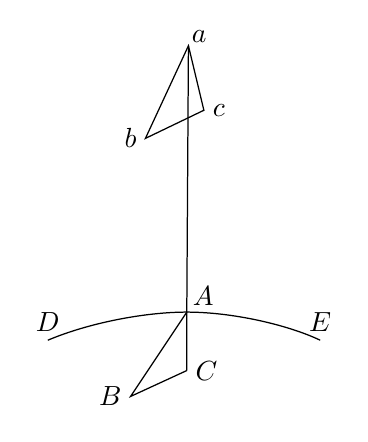
\begin{tikzpicture}[x=.007cm,y=-.007cm,line width=.45pt]
\coordinate (a) at (398,80);
\coordinate (b) at (320,248);
\coordinate (c) at (426,197);
\coordinate (A) at (395,563);
\coordinate (B) at (293,716);
\coordinate (C) at (395,669);
\draw (a)--(A)--(C);
\draw (a)--(b)--(c)--cycle;
\draw (A)--(B)--(C);
\draw (143,614) .. controls (216,583) and (318,563) .. (A)
 .. controls (478,563) and (578,586) .. (637,614);
\node[anchor=south west,inner sep=1pt] at (a) {$a$};
\node[anchor=east,inner sep=3pt] at (b) {$b$};
\node[anchor=west,inner sep=3pt] at (c) {$c$};
\node[anchor=south west,inner sep=2pt] at (A) {$A$};
\node[anchor=east,inner sep=3pt] at (B) {$B$};
\node[anchor=west,inner sep=3pt] at (C) {$C$};
\node[anchor=south,inner sep=3pt] at (143,614) {$D$};
\node[anchor=south,inner sep=3pt] at (637,614) {$E$};
\end{tikzpicture}
\end{center}
Allein dies ist \textls[150]{nicht ausreichend}, um über die Verschiedenheit der in $A$ und $a$ beobachteten Richtung der Schwere (Lothlinie) gegen den Äquator zu urtheilen, da man nicht berechtigt ist anzunehmen, dass $ab$ mit $AB$ parallel sei; in der That ist die Ungleichheit der Richtungen von $ab$ und $AB$ von derselben Ordnung, wie die aus den zwei von Ihnen angeführten Ursachen entspringende Ungleichheit der Winkel $BAC$ und $bac$. Nach einem blossen Aperçu würde man geneigt sein, zu vermuthen, dass die beiden Geraden $AB$ und $ab$, auf beiden Seiten indefinite fortgesetzt, sich nicht oben, sondern unten schneiden müssten, in welchem Falle dann diese dritte Ursache in demselben Sinne wirken würde, nemlich die Polhöhe in $a$ grösser zu machen als in $A$. Allein eine tiefer eindringende Untersuchung zeigt, dass diese Präsumption falsch ist, und dass $ab$ mit $aAC$ einen grössern und nicht einen kleinern Winkel macht als $AB$ mit $AC$, daher also diese dritte Ursache den beiden ersten \textls[150]{entgegen} wirkt und es auf das Quantitative ankommt, um sicher zu werden, ob nicht gar die Polhöhe in $a$ kleiner wird als in $A$.

Zu einer solchen Untersuchung fehlte mir nun damals die Zeit, auch abgesehen von einem nicht günstigen Gesundheitszustande. Jedoch habe ich, sobald ich es möglich machen konnte, die Untersuchung für den Fall, wo die Erde wie homogen betrachtet wird, durchgeführt. Das Resultat war, dass die Polhöhe in $a$ um
\[
206\,265''\cdot\frac s{a_0}\sin2\varphi\cdot K
\]
grösser ist als in $A$, wo $a_0$ den Halbmesser des Äquators, $s$ die Höhe $Aa$

\clearpage
\noindent\mbox{}\hfill ÄNDERUNG DER POLHÖHE MIT DER HÖHE.\hfill 101\par
\noindent in obiger Figur, $\varphi$ die Polhöhe in $A$, und $K$ einen Coefficienten bedeutet, der aber in der Voraussetzung der Homogeneität schlechthin der Abplattung gleich wird $=\theta$, übrigens aber eben nur auf die erste Ordnung der Abplattung genau ist, was jedenfalls hier vollkommen zureicht. Ich bemerke noch, dass dies $K$ wie aus drei Theilen zusammengesetzt betrachtet werden kann: $+\tfrac25\theta$ in Folge des Umstandes, dass $bc>BC$; $+\tfrac45\theta$ in Folge des Umstandes, dass $ab<AB$ und $-\tfrac15\theta$ in Folge des Nichtparallelismus von $ab$ und $AB$. Ich wollte Ihnen jedoch dies Resultat nicht gleich mittheilen, weil ich wünschte, die Untersuchung von der Voraussetzung der Homogeneität der Erde unabhängig zu machen. Ganz unabhängig von aller Voraussetzung ist es natürlich nicht möglich, ein Resultat zu erhalten. Meiner weitern Untersuchung sollte aber weiter keine Voraussetzung zum Grunde liegen, als diejenige, der (in einer oder andern Form) der berühmte \textsc{Clairaut}sche Lehrsatz
\[
\tfrac52\frac hg=\theta+\frac{g'-g}g
\]
zum Grunde liegt, wo $g$ und $g'$ die Schwere am Äquator und Pol und $h$ die Centrifugalkraft am Äquator bedeuten. Die Gültigkeit dieses Lehrsatzes ist nemlich abhängig davon, dass man entweder den Erdkörper aus ähnlichen Schichten zusammengesetzt sich vorstellt (Dichtigkeit in allen Punkten Einer Schicht dieselbe, aber in verschiedenen Schichten beliebig ungleich) oder auch bloss annimmt, die Erde sei ein elliptisches Sphäroid, oder drittens auch nur, dass der Zuwachs der Pendellänge vom Äquator zum Pol dem Quadrate des Sinus der Polhöhe proportional sei. Alles übrigens, indem man Grössen der zweiten Ordnung der Abplattung ignorirt.

Diese weitere Untersuchung habe ich jetzt auch ausgeführt, freilich nicht gerade in der Form einer Zusammensetzung des Resultats aus den gedachten drei Theilen, die sich aber doch darin wiederfinden lassen. Diese drei Theile verhalten sich hier aber nicht mehr wie die Zahlen $+2$, $+4$, $-1$, sondern die dritte wird einem complicirtern Ausdruck entsprechen. Das Endresultat wird aber merkwürdigerweise sehr einfach, nemlich
\[
K=\frac{g'-g}g,
\]
welches also das vorhergehende specielle unter sich begreift, da bekanntlich bei homogener Zusammensetzung des Erdkörpers
% Continues on printed 102.
